% =========================================================================== %
% Yes. This is a document.

\documentclass[
	english,
	aspectratio=169,
	table
]{beamer}

% =========================================================================== %
% Theme
\usepackage{scrlfile}
	\ReplacePackage{beamerthemeSHUR}{./sty/beamerthemeSHUR}
	\ReplacePackage{beamerinnerthemefancy}{./sty/beamerinnerthemefancy}
	\ReplacePackage{beamerouterthemedecolines}{./sty/beamerouterthemedecolines}
	\ReplacePackage{beamercolorthemechameleon}{./sty/beamercolorthemechameleon}

\usetheme[
	pageofpages=/,
	bullet=circle,
	titleline=true,
	alternativetitlepage=true,
	watermark="",
	watermarkheight=0px,
	watermarkheightmult=0
	]
{SHUR}

% =========================================================================== %
% the usual stuff

\usepackage[utf8]{inputenc}
\usepackage[T1]{fontenc}
\usepackage{babel}
\usepackage{lmodern}
\usepackage{microtype}
\usepackage{csquotes}
\usepackage{xspace}

\usepackage{tabularx}
\usepackage{booktabs}
\usepackage{multirow}

\usepackage{color, colortbl}
\usepackage{xcolor}
	\definecolor{tabhighlight}{RGB}{230,240,255}

\usepackage{tabto}
\usepackage{setspace}

\usepackage{minted}
	\usemintedstyle{friendly}

\usepackage{tikz}
	\usetikzlibrary{positioning}
	\usetikzlibrary{matrix}
	\usetikzlibrary{shapes.geometric}
	\usetikzlibrary{backgrounds}
	\usetikzlibrary{calc}
	\usetikzlibrary{decorations.pathreplacing}
	\tikzstyle{every picture}+=[remember picture] 
\usepackage{adjustbox}

\usepackage{amsmath}
\usepackage{physics}

\usepackage[most]{tcolorbox}
	\tcbsetforeverylayer
		{colback=cyan!10!white,
		 colframe=cyan!75!black,
		 arc=0pt,
		 outer arc=0pt
		}
	\newtcolorbox{codebox}[1][Code]
		{colback=black!5!white,
		 colframe=blue!40!black,
		 title=#1,
		 leftupper=6mm
		}
	\newtcolorbox{cmdbox}[1][Command Line]
		{colback=black,
		 coltext=white,
		 fontupper=\ttfamily ,
		 colframe=blue!40!black,
		 title=#1,
		 outer arc=0pt
		}
	\newtcolorbox{warnbox}[1][Warning]
		{colback=black!5!white,
		 colframe=red!40!black,
		 title=#1
		}
	\newtcolorbox{hintbox}[1][Hint]
		{colback=black!5!white,
		 colframe=green!40!black,
		 title=#1
		}
	\newtcolorbox{defbox}[1][Code]
		{colback=cyan!10!white,
		 colframe=cyan!90!black,
		 title=#1
		}
	\newtcolorbox{recapbox}[1][Code]
		{colback=yellow!10!white,
		 colframe=yellow!90!black,
		 coltitle=black,
		 title=#1
		}
%==============================================================================%
% GLOBAL MACROS

\newcommand*{\zB}{e.\,g. }
\newcommand*{\ie}{i.\,e. }

\newcommand{\Thus}{\ensuremath{\Rightarrow}\xspace}
\newcommand{\thus}{\ensuremath{\rightarrow}\xspace}

\newcommand*{\tabcrlf}{\\ \midrule}			% actually still allows for optional argument

\newcommand*{\inPy}[1]{\mintinline{python}{#1}}

\newcommand*{\todo}[1]{{\color{red}TODO: #1}}
\newcommand*{\sfrac}[2]{\ensuremath{{}^{#1}/_{#2}}}

% =========================================================================== %

\author{Stefan Hartinger}
\title{Python for Scientists}
\subtitle{Part 21: The Hypertext Transfer Protocol (HTTP)}
\institute{Department of Just Some Dude Who Likes to Talk}
\date{Winter 2023/24}

% =========================================================================== %

\begin{document}
\newcommand{\rx}[1]{\texttt{"{\color{olive}#1}"}}
\newcommand{\match}[1]{{\color{blue}#1}}
\newcommand{\qtt}[1]{\texttt{"{#1}"}}

% =========================================================================== %

\begin{frame}[t,plain]
\titlepage
\end{frame}

% =========================================================================== %

\begin{frame}[fragile]{Red Line Through HTTPS}
%
\begin{center}
\begin{columns}
\column{.45\linewidth}
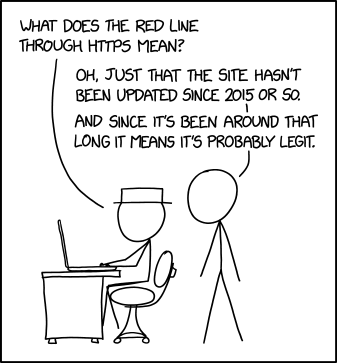
\includegraphics[width=.9\linewidth]{./gfx/21-xkcd-red_line_through_https}
%
\column{.45\linewidth}
\emph{Some organization has been paying to keep this up and it hasn't been removed from search results. Seems like two votes of confidence to me.}

\vspace{6pt}
Source: \url{https://xkcd.com/2634/}

\end{columns}
\end{center}
%
\end{frame}

% =========================================================================== %

\begin{frame}{Scope For Today}
%
\begin{itemize}
\item Recap
\item HTTP and HTTPS
	\begin{itemize}
	\item Requests
	\item Status Codes
	\item HTTP Headers
	\item MIME-Types and encoding
	\end{itemize}
\item Python's \texttt{http} and \texttt{urllib}
\end{itemize}
%
\end{frame}

% =========================================================================== %

\begin{frame}{Recap}
%
\begin{itemize}
\item OSI Layers: 7 abstraction levels describing different aspects of network communication
	\begin{itemize}
	\item Layer 3: IP layer -- finding a route through a network
		\begin{itemize}
		\item IP addresses identify a host
		\item Domains resolved by DNS server
		\end{itemize}
\pause
	\item Layer 4: Transport layer -- makes communication reliable
		\begin{itemize}
		\item TCP (Transmission Control Protocol): messages arrive in order and are known to arrive
		\item UDP (User Datagram Protocol): lightweight/low traffic protocol without safety features 
		\end{itemize}
\pause
	\item Layer 5: Session layer -- allows multiple mesages back and forth
		\begin{itemize}
		\item Sockets, see last lecture
		\item Most often used for only one request and one answer before being discarded
		\end{itemize}
\pause
	\item Layer 6: Representation layer -- how to encode information in a bytestream
		\begin{itemize}
		\item XML, JSON, ...
		\end{itemize}
\pause
	\item Layer 7: Application layer -- APIs for what you actually want to do in the first place
		\begin{itemize}
		\item Email protocols SMTP, POP3; Domain Name Service (DNS); File Transport Protocol (FTP)
		\item HTTP, HTTPS
		\end{itemize}
	\end{itemize}
\end{itemize}
%
\end{frame}

% =========================================================================== %

\begin{frame}{HTTP and HTTPS}
%
\begin{itemize}
\item HyperText Transfer Protocol (Secure)
	\begin{itemize}
	\item Both: designed for exchange of human readable text, but capable of transmitting arbitrary binary data
	\item HTTPS is HTTP plus TLS/SSL (Transport Layer Security/Secure Sockets Layer): cryptographic protocols somewhere between layers 4 and 6
	\item Ports 80/8080 (HTTP) and 443/8443 (HTTPS)
	\item Clear distinction between server and client: client sends \emph{requests}, server sends \emph{responses}
	\end{itemize}
\pause
\item Properties
	\begin{itemize}
	\item Stateless: peers only know about each other for only one request/response (as far as HTTP is concerned).
		In principle, a first message cannot be distinguished from a subsequent message
	\item Connectionless: a socket is used for only one request/response cycle.\\
		(However, to improve performance, there is a mechanism to keep sockets for more than one exchange...)
	\item Media independent: any data can be sent as long as peers know how to handle it.
	\end{itemize}
\end{itemize}
%
\end{frame}

% =========================================================================== %

\begin{frame}{HTTP Messages}
%
\begin{tcbraster}[raster columns=2,
                  raster equal height,
                  nobeforeafter,
                  raster column skip=0.1cm]
\begin{codebox}[Request Structure]
\ttfamily
REQUEST TYPE LINE \\
HEADER \\
\\
BODY
\end{codebox}
%
\begin{codebox}[Response Structure]
\ttfamily
RESPONSE TYPE LINE \\
HEADER \\
\\
BODY
\end{codebox}
\end{tcbraster}
%
\begin{itemize}
\item Each line corresponds to an actual printable line
\item Line breaks are specified as CRLF (\inPy{"\r\n"})
\item First line gives context how to interpret the rest
	\begin{itemize}
	\item Examples: GET request: please send the document under \texttt{/website/index.html}
	\item Example: OK response: you'll find the file content in the \texttt{BODY}
	\end{itemize}
\item \texttt{HEADER} and \texttt{BODY} may be zero to multiple lines long
\item The empty line between \texttt{HEADER} and \texttt{BODY} is used to distinguish \texttt{HEADER} from \texttt{BODY}
\end{itemize}
%
\end{frame}

% =========================================================================== %

\begin{frame}{Request Lines}
%
\begin{codebox}[Request Line Structure]
\ttfamily
METHOD [space] URI [space] HTTP-VERSION
\end{codebox}
%
\begin{itemize}
\item \texttt{METHOD} is a case sensitive and always uppercase word
	\begin{itemize}
	\item \texttt{GET}: Please send the file specified by \texttt{URI}
	\item \texttt{HEAD}: Please send only the header for \texttt{GET URI}
	\item \texttt{POST}: In \texttt{BODY} you will find information to process according to \texttt{URI}
	\item \texttt{PUT}: Please write \texttt{BODY} to \texttt{URI}
	\item \texttt{DELETE}: Please delete \texttt{URI}
	\item \texttt{CONNECT}: Forward all subsequent requests unchanged to \texttt{URI} (\thus \emph{proxy-server})
	\item \texttt{TRACE}: Please send this message back to me (for testing connectivity)
	\item \texttt{OPTIONS}: Please tell me which \texttt{METHOD}s you allow
	\end{itemize}
\item Note: for security reasons, most servers only allow \texttt{GET} and maybe \texttt{POST}
\end{itemize}
%
\end{frame}

% =========================================================================== %

\begin{frame}
%
\begin{codebox}[URI Structure]
\ttfamily
[DOMAIN] ABSOLUTE\_PATH [PARAMETERS] | "*" 
\end{codebox}
%
\begin{itemize}
\item URI: Unique Resource Identifier -- unambiguous description of what \texttt{METHOD} applies to
\item \texttt{ABSOLUTE\_PATH}: Syntax of a Linux file path
	\begin{itemize}
	\item Usually actually identifies a file on the server, but may have arbitrary meaning
	\item Example \texttt{POST}: may identify a subroutine on the server
	\end{itemize}
\item \texttt{DOMAIN}: used when communicating via proxy servers
\item \texttt{PARAMETERS}: 
	\begin{itemize}
	\item Sequence of \texttt{KEY=VALUE} separated by ampersand (\&)
	\item Initiated by question mark (?)
	\item Example: \texttt{{\color{gray}https://music.youtube.com}{\color{cyan}/watch}{\color{purple}?}{\color{blue}v=LUzKawNZ-rA}{\color{purple}\&}{\color{blue}list=RDAMVMb-vx8PpL8Gg}}
	\end{itemize}
\item Asterisk (\texttt{*}): no particular resource, the server itself
	\begin{itemize}
	\item Usually only for \texttt{OPTIONS}
	\end{itemize}
\end{itemize}
%
\end{frame}

% =========================================================================== %

\begin{frame}[fragile]
%
\begin{codebox}[HTTP-VERSION Structure]
\ttfamily
"HTTP/1." VERSION
\end{codebox}
%
\begin{itemize}
\item Currently in use are versions 1.1, 1.2 and 1.3
	\begin{itemize}
	\item Structure of messages remains the same
	\item Additional allowed \texttt{HEADER} fields in newer versions
	\item HTTP/2 (aka HTTP/1.2)
		\begin{itemize}
		\item Introduces data compression (\zB gzip)
		\item Introduces \emph{server push}: server sends data without prior request (\zB website HTML and referenced images)
		\item Supported by 97\% of all web browser installations
		\end{itemize}
	\item HTTP/3 (aka HTTP/1.3)
		\begin{itemize}
		\item Replaces TCP/TLS 1.2 with QUIC/TLS 1.3, which is UDP-based
		\item A lot faster
		\item Supported by 94\% of all web browser installations
		\end{itemize}
	\end{itemize}
\item For most concerns: regard as equal
\end{itemize}
%
\end{frame}

% =========================================================================== %

\begin{frame}{Message Headers}
%
\begin{codebox}[HEADER Line Structure]
\ttfamily
FIELD\_NAME: VALUE
\end{codebox}
%
\begin{itemize}
\item \texttt{FIELD\_NAME}:
	\begin{itemize}
	\item Case insensitive, usually Title Case or all lower case
	\item May not contain whitespaces; words usually separated by hyphens (\zB \texttt{Content-Language})
	\item Leading whitespaces are ignored
	\end{itemize}
\item Categorized into
	\begin{itemize}
	\item Request-header: may only meaningfully appear in client requests
	\item Response-header: may only meaningfully appear in server responses
	\item General-header: equally valid in requests and responses
	\item Entity-header: contain metadata about the message-body or requested resource
	\end{itemize}
\item Standardized, but web applications may define arbitrary extensions
\end{itemize}
%
\end{frame}

% =========================================================================== %

\begin{frame}{Common Header Fields}
%
\begin{itemize}
\item Entity Headers
	\begin{itemize}
	\item \texttt{Content-Length}: The size of the resource, in decimal number of bytes.
	\item \texttt{Content-Type}: (aka MIME-Type; see later) Indicates the media type of the resource.
	\item \texttt{Content-Encoding}: Used to specify the compression algorithm.
	\item \texttt{Content-Language}: Describes the human language(s) intended for the audience, so that it allows a user to differentiate according to the users' own preferred language.
	\end{itemize}
\item File Handling
	\begin{itemize}
	\item \texttt{Content-Disposition}: tells whether to treat \texttt{BODY} as download or HTML to be displayed
	\end{itemize}
\item Cookies
	\begin{itemize}
	\item \texttt{Set-Cookie}: pairs of \texttt{key=value} to persist on the client site for various purposes, \zB session management, personalization or tracking
	\end{itemize}
\item Caching
	\begin{itemize}
	\item \texttt{Vary}: tells which parts of the header influenced the result (\ie need to be stored when caching)
	\end{itemize}
\end{itemize}
%
%https://developer.mozilla.org/en-US/docs/Web/HTTP/Headers
%
\end{frame}

% =========================================================================== %

\begin{frame}{MIME-Types}
%
\begin{itemize}
\item MIME-Types
	\begin{itemize}
	\item Multipurpose Internet Mail Extensions
	\item String identifying how to interpret data
	\item Form \texttt{family/subtype}
	\item \texttt{family}: one from \texttt{application}, \texttt{audio}, \texttt{font}, \texttt{image}, \texttt{model}, \texttt{text}, \texttt{video}
	\item \texttt{subtype} depends on \texttt{family} and lists virtually any file type
	\item E.\;g. \texttt{text/html}, or \texttt{application/octet-stream} for raw/untyped binary data
	\item \texttt{subtype} may
	\end{itemize}
\pause
\item Parametrized MIME-Types
	\begin{itemize}
	\item Extended form: \texttt{{\color{gray}family/subtype}{\color{purple};parameter=value}}
	\item Often: \texttt{charset=CHARSET}
	\item \texttt{CHARSET}: \texttt{utf-8}, \texttt{ascii}, \texttt{iso-8859-1}, ...
	\end{itemize}
\pause
\item Learn more about this here:
	\begin{itemize}
	\item \url{developer.mozilla.org/en-US/docs/Web/HTTP/Basics_of_HTTP/MIME_types}
	\end{itemize}
\end{itemize}
%
\end{frame}

% =========================================================================== %

\begin{frame}[fragile]{Message Body, MIME-Types}
%
\begin{itemize}
\item \texttt{BODY}
	\begin{itemize}
	\item Arbitrary data, content defined by context of communication (Webbrowser, App, ...)
	\item Transfers the payload (\zB the website, a file to download, ...)
	\end{itemize}
\pause
\item Form-Data
	\begin{itemize}
	\item Think of data for a web-app, \zB a bus connection timetable
	\item Often, instrucitons how to identify fields is given in \texttt{Content-Type} header field
\pause
	\item Example:
		\begin{minted}[fontsize=\scriptsize]{text}
Content-Type: multipart/form-data;boundary="boundary"

--boundary
Content-Disposition: form-data; name="field1"

value
--boundary
Content-Disposition: form-data; name="field2"; filename="example.txt"

file contents
--boundary--
		\end{minted}
	\end{itemize}
\end{itemize}
%
\end{frame}

% =========================================================================== %

\begin{frame}{Server Response Lines}
%
\vspace{-9pt}
\begin{codebox}[Server Response Line Structure]
\ttfamily
HTTP-VERSION [space] STATUS\_CODE [space] REASON
\end{codebox}
%
\vspace{-6pt}
\begin{itemize}
\item \texttt{HTTP\_VERSION}: same as for client requests
\pause
\item \texttt{STATUS\_CODE}: three-digit integer; \texttt{REASON}: string, human readable equivalent
	\begin{itemize}
	\item 100 - 199: informational responses (like \texttt{100 Continue}: server has sent partial data and client should request more)
	\item 200 - 299: success messages (like \texttt{200 OK}: the request has been processed; see \texttt{HEADER} and \texttt{BODY} for results)
	\item 300 - 399: redirection messages (like \texttt{302 Permanently Moved}: the ressource has a new URI which the client should request and remember)
	\item 400 - 499: client error messages (like \texttt{404 Not Found}: the requested ressource does not exist on the server)
	\item 500 - 599: server error messages (like \texttt{501 Not Implemented}: the request is valid HTTP, but the server does not know how to respond to this)
	\end{itemize}
\end{itemize}
%
\end{frame}

% =========================================================================== %

\begin{frame}[fragile]
%
\vspace{-8pt}
\begin{cmdbox}[Example Response from Wikipedia]
\begin{minted}[fontsize=\tiny]{text}
HTTP/2 200 
date: Wed, 11 Oct 2023 19:34:02 GMT
last-modified: Tue, 03 Oct 2023 20:18:39 GMT
content-language: de
content-type: text/html; charset=UTF-8
vary: Accept-Encoding,Cookie
server: ATS/9.1.4
x-content-type-options: nosniff
x-cache: cp3071 hit, cp3071 miss
x-cache-status: hit-local
x-client-ip: 2003:e9:af0a:6a00:48fa:3502:55f5:5afb
...
set-cookie: WMF-Last-Access=11-Oct-2023;Path=/;HttpOnly;secure;Expires=Sun, 12 Nov 2023 12:00:00 GMT
set-cookie: WMF-Last-Access-Global=11-Oct-2023;Path=/;Domain=.wikipedia.org;HttpOnly;secure;
            Expires=Sun, 12 Nov 2023 12:00:00 GMT
set-cookie: WMF-DP=bc8;Path=/;HttpOnly;secure;Expires=Thu, 12 Oct 2023 00:00:00 GMT
set-cookie: GeoIP=DE:BY:Regensburg:49.01:12.07:v4; Path=/; secure; Domain=.wikipedia.org
set-cookie: NetworkProbeLimit=0.001;Path=/;Secure;Max-Age=3600
cache-control: private, s-maxage=0, max-age=0, must-revalidate
accept-ranges: bytes
content-length: 188221

<!DOCTYPE html>
<html class="client-nojs" lang="de" dir="ltr">
<head>
<meta charset="UTF-8">
<title>Universität Regensburg – Wikipedia</title>
...
\end{minted}
\end{cmdbox}

\begin{minted}[fontsize=\tiny]{text}
\end{minted}
%
\end{frame}

% =========================================================================== %

\begin{frame}{Tangent: CURL}
%
\begin{itemize}
\item \texttt{curl}: Linux Command Line Tool for manually making HTTP requests
	\begin{itemize}
	\item Can be installed from the default repositories
	\item Windows: \texttt{https://curl.se/windows/}
	\end{itemize}
\item Last slide from\\
	\texttt{curl -i https://de.wikipedia.org/wiki/Universität\_Regensburg}
	\begin{itemize}
	\item Option \texttt{-i}: include headers
	\item Option \texttt{-d <data>}: make a \texttt{POST} request
	\end{itemize}
\item Though you'll like the Python interface better ;)
\end{itemize}
%
\end{frame}

% =========================================================================== %

\begin{frame}{Going Python: \texttt{http} and \texttt{urllib}}
%
\begin{itemize}
\item \texttt{http}
	\begin{itemize}
	\item Low level package for client/server requests
	\item Submodules \texttt{client}, \texttt{server}, \texttt{cookies} and \texttt{cookiejar}
	\item Enums \texttt{HTTPStatus} and \texttt{HTTPMethod}
	\end{itemize}
\pause
\item \texttt{urllib}
	\begin{itemize}
	\item Built upon \texttt{http}, more convenient to use for client side requests
	\item Uses HTTP/1.1
	\item Mostly client side functions
	\item Submodules \texttt{request}, \texttt{error}, \texttt{parse} and \texttt{robotparser}
\pause
		\begin{itemize}
		\item Webeservers often offer a \texttt{robots.txt}
		\item This is requested by search engines, not humans
		\item Helps reducing webtraffic
		\item \texttt{urllib.robotparser} helps with reading these files
		\end{itemize}
	\end{itemize}
\end{itemize}
%
\end{frame}

% =========================================================================== %

\begin{frame}[fragile]{Client side: \texttt{urllib.request}}
%
\begin{itemize}
\item Function \inPy{urlopen(url, data=None, timeout=None, ssl_args=None)}
	\begin{itemize}
	\item \texttt{url}:
		\begin{itemize}
		\item Either a \inPy{str}ing \Thus address of the webserver to reach \\
			results in a \texttt{GET} request if \texttt{data} is \inPy{None} or \texttt{POST} otherwise
		\item Or a \texttt{Request} object (see next slide) \Thus arbitrary request, more control over headers
		\end{itemize}
	\item \texttt{data}: a \inPy{bytes} object used with \texttt{POST} requests
	\item \texttt{timeout}: maximum time in seconds to wait before \inPy{raise}ing an error
	\item \texttt{ssl\_args}: actually \texttt{cafile}, \texttt{capath}, \texttt{cadefault}, \texttt{context}: Used for SSL-encrypted connections
	\end{itemize}
\pause
\item Returns a \texttt{http.client.HTTPResponse} object
	\begin{itemize}
	\item Attributes \texttt{status}, \texttt{msg} and \texttt{reason} -- server response line (\zB \texttt{200 OK})
	\item Method \texttt{getheaders()} -- all headers as a \inPy{list} of 2-\inPy{tuple}s
	\item Method \texttt{read(amount)} -- read up to \texttt{amount} bytes from \texttt{BODY}
		\begin{itemize}
		\item \texttt{amount} can be omitted -- reads the whole \texttt{BODY}
		\end{itemize}
	\item Context manager object -- can be used in a \inPy{with} block
	\end{itemize}
\end{itemize}
%
\end{frame}

% =========================================================================== %

\begin{frame}{The \texttt{Request} Object}
%
\begin{itemize}
\item \inPy{Request(url, data, headers, origin_req_host, unverifiable, method)}
	\begin{itemize}
	\item \texttt{url}: \inPy{str}ing, complete with protocol (\texttt{{\color{purple}https://}{\color{gray}de.wikipedia.org}})
	\item \texttt{data}: \inPy{bytes}-Object to be sent (imples \inPy{method="GET"}). Defaults to \inPy{None}
	\item \texttt{headers}: \inPy{dict} of HTTP headers. Defaults to empty \inPy{dict}
	\item \texttt{origin\_req\_host}: Host name or IP of original requester if using proxies. \\
		Defaults to \inPy{None}
	\item \texttt{unverifiable}: whether the user explicitly requested this object. Defaults to \inPy{False}\\
		Example: when loading a homepage, you explicitly request the HTML document, but only implicitly the images referred to by the HTML document.
	\item \texttt{method}: one of the HTTP methods
	\end{itemize}
\pause
\item Useful methods and attributes
	\begin{itemize}
	\item \texttt{get\_method()}
	\item \texttt{add\_header(key, value)}, \texttt{remove\_header(key)}
	\item \texttt{has\_header(key)}, \texttt{header\_items()}
	\item \texttt{data}
	\end{itemize}
\end{itemize}
%
\end{frame}

% =========================================================================== %

\begin{frame}[fragile]{URL Encoding and Helpers}
%
\begin{itemize}
\item URIs/URLs are ASCII-only
	\begin{itemize}
	\item Note: URIs (Uniform Resource Identifyer) is the superset of 
	URL (Uniform Resource Locator, used for file-like objects) and URNs (Uniform Resource Name; \zB ISBN-Codes)
	\end{itemize}
\pause
\item 2005: Introduction of IRIs (\emph{International Resource Identifiers})
	\begin{itemize}
	\item Just like URIs, but allow Unicode characters
	\item Mapping to ASCII-Only URIs via \emph{percent encoding}
	\end{itemize}
\pause
\item Helper functions to do the dirty work for you in \texttt{urllib.parse}
	\begin{itemize}
	\item \inPy{quote(string, safe='/', encoding='utf-8')} -- Unicode to ASCII
		\begin{itemize}
		\item \texttt{string}: what to encode; may be a \inPy{str}ing or a \inPy{bytes} object
		\item \texttt{safe}: ASCII characters that should NOT be encoded
		\item \texttt{encoding}: used when parsing a \inPy{bytes} object
		\end{itemize}
	\item \inPy{unquote(string, encoding='utf-8')} -- ASCII to Unicode
	\end{itemize}
\end{itemize}
%
\end{frame}

% =========================================================================== %

\begin{frame}[fragile]
%
\vspace{-6pt}
\begin{codebox}[Downloading A Website ...]
\begin{minted}[fontsize=\scriptsize, linenos]{python3}
from http import HTTPStatus
import urllib.request as ur
import urllib.error   as ue
from urllib.parse import quote

HOST = "https://de.wikipedia.org/wiki/" + quote("Universität Regensburg")
MAX_LINES_TO_SHOW = 5

try:
    with ur.urlopen(HOST) as f:
        if (f.status == HTTPStatus.OK):
            headers = dict(f.getheaders())
            for key, value in headers.items():
                print(f"{key:25}: {value}")
            print()
            encoding = get_charset(headers)      # see next slide for get_charset
            data_lines = f.read().decode(encoding).splitlines()
            lines_to_show = min(MAX_LINES_TO_SHOW, len(data_lines))
            for line in data_lines[:lines_to_show]:
                print(line)
\end{minted}
\end{codebox}
%
\end{frame}

% =========================================================================== %

\begin{frame}[fragile]
%
\vspace{-6pt}
\begin{codebox}[... continued]
\begin{minted}[fontsize=\scriptsize, linenos, firstnumber=last]{python3}
        else:
            print(f"Unexpected non-error response when requesting '{HOST}':")
            print(f.reason)

except ValueError as e:
    print(f"Could not resolve URL '{HOST}'")
    print(f"Reason: {e}")  # e.g. unknown url type: when omitting the protocol
except ue.HTTPError as e:
    print(f"An error occurred while loading '{HOST}':")
    print(e)               # e.g. HTTP Error 404: Not Found


def get_charset(headers:dict[str, str]):
    content_type = headers['content-type']
    elements = content_type.split(';')
    if len(elements) == 1:
        return 'ascii'
    else:
        content_type_parameters = dict(foo.strip().split('=') for foo in elements[1:])
        return content_type_parameters.get('charset', 'ascii')
\end{minted}
\end{codebox}
%
\end{frame}

% =========================================================================== %

\begin{frame}[fragile]
%
\vspace{-6pt}
\begin{cmdbox}[Output]
\begin{minted}[fontsize=\tiny]{text}
date                     : Sun, 15 Oct 2023 03:24:06 GMT
vary                     : Accept-Encoding,Cookie
server                   : ATS/9.1.4
x-content-type-options   : nosniff
content-language         : de
accept-ch                : 
last-modified            : Tue, 03 Oct 2023 20:18:39 GMT
content-type             : text/html; charset=UTF-8
age                      : 27776
x-cache                  : cp3070 miss, cp3070 hit/2
x-cache-status           : hit-front
server-timing            : cache;desc="hit-front", host;desc="cp3070"
strict-transport-security: max-age=106384710; includeSubDomains; preload
report-to                : { "group": "wm_nel", "max_age": 604800, ...
nel                      : { "report_to": "wm_nel", "max_age": 604800, "failure_fraction": 0.05, ...
set-cookie               : NetworkProbeLimit=0.001;Path=/;Secure;Max-Age=3600
x-client-ip              : 2003:e9:af0a:6a00:d4cd:8d4d:485f:de7
cache-control            : private, s-maxage=0, max-age=0, must-revalidate
accept-ranges            : bytes
content-length           : 188248
connection               : close

<!DOCTYPE html>
<html class="client-nojs" lang="de" dir="ltr">
<head>
<meta charset="UTF-8">
<title>Universität Regensburg – Wikipedia</title>
\end{minted}
\end{cmdbox}
%
\end{frame}

% =========================================================================== %

\begin{frame}{Python HTTP-Server: \texttt{http.server}}
%
\begin{warnbox}[From the Python Docs]
\footnotesize
Warning: \texttt{http.server} is not recommended for production. It only implements basic security checks.
\end{warnbox}
%
\begin{itemize}
\item Module provides basic infrastructure for handling HTTP requests
\item Class \texttt{HTTPServer} -- abstracts away the sockets work
	\begin{itemize}
	\item You'll usually only instantiate one and call \texttt{instance.serve\_forever()}
	\end{itemize}
\item Class \texttt{BaseHTTPRequestHandler}
	\begin{itemize}
	\item Base class, contains stubs for each HTTP request
	\item Inherit from and define server responses here
	\item Methods \texttt{do\_<METHOD>} (\zB \texttt{do\_GET}, \texttt{do\_POST})
	\item If not overridden, automatically answers with 501: Not implemented plus HTML error message for humans/webbrowsers
	\end{itemize}
\end{itemize}
%
\end{frame}

% =========================================================================== %

\begin{frame}{Minimal Setup: \texttt{HTTPServer}}
%
\begin{itemize}
\item Constructor: \texttt{HTTPServer(server\_address, RequestHandlerClass)}
	\begin{itemize}
	\item \texttt{server\_address} -- \texttt{tuple} of IP address and port under which the server can be reached
		\begin{itemize}
		\item Given as a \inPy{str}ing
		\item May be an empty \inPy{str}ing (accept all connections)
		\item May also be a domain like \inPy{'localhost'}; domain must be known to the OS
		\end{itemize}	
	\item \texttt{RequestHandlerClass} -- the class that will do the actual work
		\begin{itemize}
		\item Really a \texttt{class}, not an instance! \texttt{HTTPServer} will instantiate a new handler for each request!
		\end{itemize}
	\end{itemize}
\pause
\item Method \inPy{serve_forever(poll_interval=0.5)}
	\begin{itemize}
	\item Checks every \texttt{poll\_intervall} seconds for new incoming requests
	\end{itemize}
\pause
\item Itself derived from \texttt{socketserver.TCPServer}
	\begin{itemize}
	\item For more details, see \texttt{https://docs.python.org/3/library/socketserver.html\#socketserver.TCPServer}
	\end{itemize}
\end{itemize}
%
\end{frame}

% =========================================================================== %

\begin{frame}[fragile]
%
\begin{tcbraster}[raster columns=2,
                  raster equal height,
                  nobeforeafter,
                  raster column skip=0.1cm]
\begin{codebox}[Minimal Code]
\begin{minted}[fontsize=\scriptsize, linenos]{python3}
import http.server as hs

PORT = 8080
Handler = hs.SimpleHTTPRequestHandler
# Note: SimpleHTTPRequestHandler is a
# predefined handler under
# BaseHTTPRequestHandler

with hs.HTTPServer(
        ("", PORT), Handler
    ) as daemon:
    print("serving at port", PORT)
    daemon.serve_forever()
\end{minted}
\end{codebox}
%
\begin{defbox}[Result]
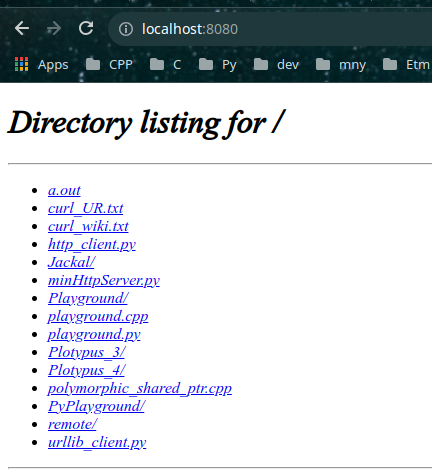
\includegraphics[width=\linewidth]{./gfx/21-SimpleHttpHandler}
\end{defbox}
\end{tcbraster}
%
\end{frame}

% =========================================================================== %

\begin{frame}{\texttt{http.server.BaseHTTPRequestHandler}}
%
\begin{itemize}
\item Request parts
	\begin{itemize}
	\item \texttt{requestline} -- the full HTTP request (\zB \texttt{GET /foo/bar HTTP/1.1})
	\item \texttt{command} -- the method (\zB \texttt{GET})
	\item \texttt{path} -- the URI in the HTTP request (\zB \texttt{/foo/bar})
	\end{itemize}
\pause
\item Payload parts
	\begin{itemize}
	\item \texttt{headers} -- \inPy{dict}-like object
	\item \texttt{rfile} -- file-like object from which the \texttt{BODY} can be read
	\item \texttt{wfile} -- file-like object; write the response \texttt{BODY} to this
	\end{itemize}
\pause
\item Sending responses
	\begin{itemize}
	\item \texttt{send\_response(code)} -- sends the response code (\zB \texttt{200 OK})
	\item \texttt{send\_header(key, value)} -- adds a single header line
	\item \texttt{end\_headers()} -- flushes the header data from a buffer to the response
	\item \texttt{wfile.write(data)} -- sends the \texttt{BODY} (\texttt{data} must be a \inPy{bytes} object)
	\item Commands must be in this oder
	\end{itemize}
\end{itemize}
%
\end{frame}

% =========================================================================== %

\begin{frame}{Print Server (Stub)}
%
\begin{columns}[T]
\column{.6\linewidth}
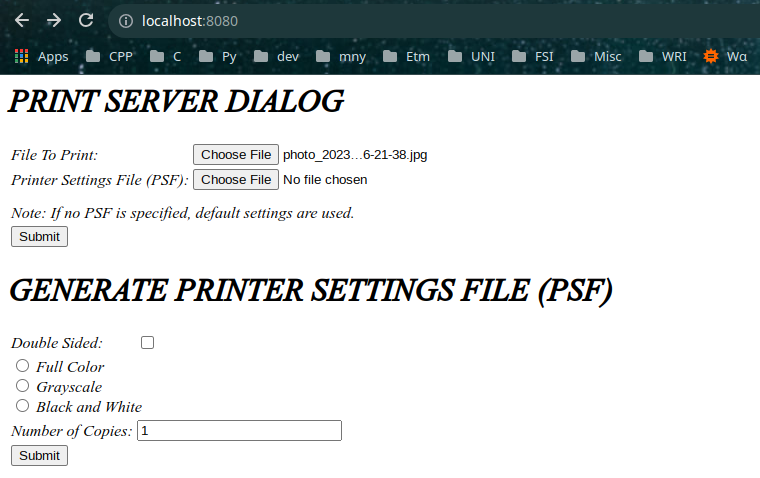
\includegraphics[width=\linewidth]{./gfx/21-printer_server}
%
\column{.3\linewidth}
For a more involved example, see the example on GRIPS.

\vspace{6pt}
You'll find that the use of the library itself is pretty straight forward

\vspace{6pt}
Most of the code deals with parsing strings or provides the right \enquote{magic constants} (\zB \texttt{text/html})
\end{columns}
%
\end{frame}

% =========================================================================== %

\begin{frame}{Links}
%
\begin{itemize}
\item Python Docs
	\begin{itemize}
	\item \url{https://docs.python.org/3/library/http.html}
	\item \url{https://docs.python.org/3/library/urllib.html}
	\item \url{https://docs.python.org/3/library/socketserver.html}
	\item \url{https://docs.python.org/3/howto/urllib2.html}
	\end{itemize}
\item Mozilla Developer Network 
	\begin{itemize}
	\item \url{https://developer.mozilla.org/en-US/docs/Web/HTTP}
	\item \url{https://developer.mozilla.org/en-US/docs/Web/HTML}
	\item \url{https://developer.mozilla.org/en-US/docs/Web} (Guidelines)
	\end{itemize}
\item Basics Tutorials
	\begin{itemize}
	\item \url{https://www.tutorialspoint.com/http/index.htm}
	\item \url{https://www.w3schools.com/whatis/whatis_http.asp}
	\end{itemize}
\end{itemize}
%
\end{frame}

% =========================================================================== %
\end{document}

% MAREI!!
% whom do I give credit? Where?